\documentclass[class=report, crop=false, 12pt,a4paper]{standalone}
\usepackage{enumitem}
\usepackage{multicol}
\usepackage{graphicx}
\usepackage{float}
\usepackage{amsmath}
\usepackage{amssymb}
\usepackage{mathtools}
\usepackage{siunitx}
\usepackage{commath}
\usepackage{array}
\usepackage{booktabs}
\usepackage{natbib}
\usepackage[a4paper,width=150mm,top=25mm,bottom=25mm]{geometry}
\usepackage{parskip}
\raggedbottom
\begin{document}
\chapter{Full fault analysis}
\section{Unbalanced impedance}
\subsection{Impedance and sequence components}
We have established that in a three-phase unbalanced network there are line and phase voltages and currents that deviate in their relationships from the balanced case. Furthermore, any unbalance can be described as a set of sequence components consisting positive, negative and zero sequence phasors. Now considering impedances in unbalanced networks then we need to ensure that we understand:
\begin{itemize}
	\item How to change between star and delta arrangements
	\item Appreciate how sequence impedance is calculated
\end{itemize}
\subsection{Unbalanced star and delta equivalence}
$Z_{delta} = 3\cdot Z_{star}$ for all three phases when the loads in the three-phase system were balanced. This was helpful when looking at symmetrical faults since we normally convert delta connections into star connections and consider an impedance diagram as representing one phase. When loads are unbalanced then we need to consider each phase independently because they are subjected to different voltages, currents and impedances. Consider the two circuits below. The star and delta equivalence must result in the same line voltages and currents. In other words the impedance between any two impedances must be equivalent.
\begin{figure}[H]
	\centering
	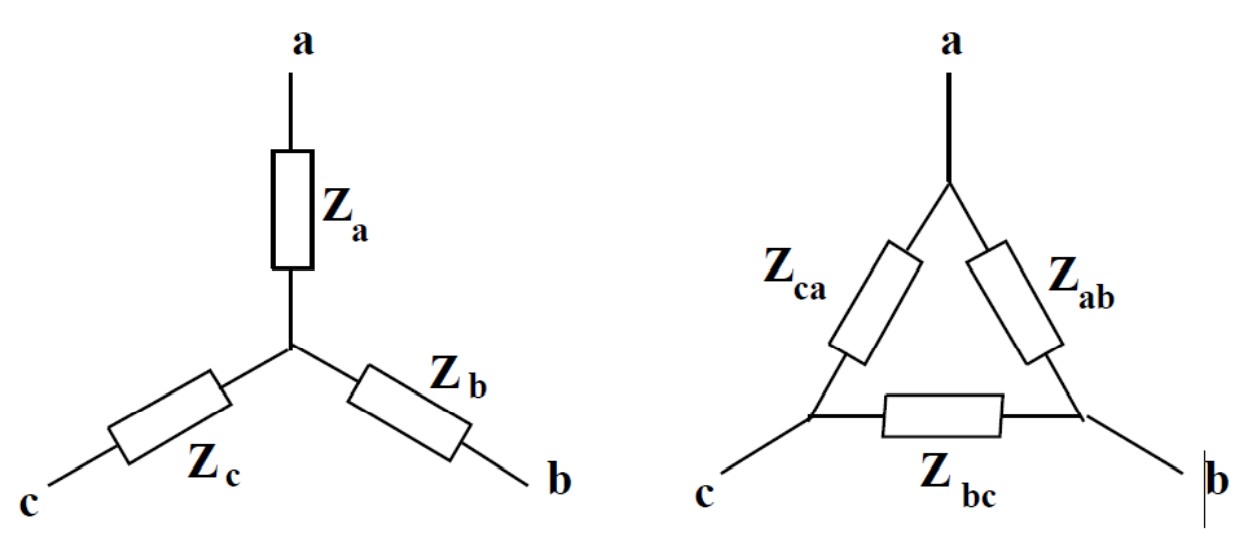
\includegraphics[width = \textwidth]{../img/figure31.png}
	\caption{Star and delta arrangements.}
\end{figure}
For example considering phase a and phase b, the impedance equivalence must be:
\begin{gather}
	Z_a + Z_b = Z_{ab} // \left(Z_{ca}+Z_{bc}\right) \textrm{ similarly,}\\
	Z_b + Z_c = Z_{bc} // \left(Z_{ab}+Z_{ca}\right)\\
	Z_c + Z_a = Z_{ca} // \left(Z_{bc}+Z_{ab}\right)
\end{gather}
By manipulation and substitution then it is possible to derive the following relationships:
\begin{gather}
	Z_{ab} = \frac{Z_aZ_b + Z_bZ_c+Z_cZ_a}{Z_c}\\
	Z_{bc} = \frac{Z_aZ_b + Z_bZ_c+Z_cZ_a}{Z_a}\\
	Z_{ca} = \frac{Z_aZ_b + Z_bZ_c+Z_cZ_a}{Z_b}
\end{gather}
and
\begin{gather}
	Z_a = \frac{Z_{ab}Z_{ca}}{Z_{ab}+Z_{bc}+Z_{ca}}\\
	Z_b = \frac{Z_{ab}Z_{bc}}{Z_{ab}+Z_{bc}+Z_{ca}}\\
	Z_b = \frac{Z_{bc}Z_{ca}}{Z_{ab}+Z_{bc}+Z_{ca}}
\end{gather}
These relationships are needed when considering impedance in unbalanced loads.
\subsection{Good practice}
In many fault calculations it is handy to convert delta impedances into star impedances because:
\begin{itemize}
	\item It ensures that all balanced arrangements are related to ground or virtual group (floating star point)
	\item When calculating faults then it is apparent that such calculations are made for one phase and then `phase shifted' to determine impact on other phases. Having everything as a star arrangement (mathematically and circuit wise) assits in ensuring that right values are obtained.
\end{itemize}
\section{Impedance of sequences}
There are positive, negative and zero phase sequence components: In voltage these are represented by $V_0$, $V_1$ and $V_2$. In current these are represented by $I_0$, $I_1$ and $I_2$.
\subsection{Sequence components and impedance}
Since $V=IZ$, it follows if there are sequence components in both voltage and current then there must be a sequence impedance too:
\begin{itemize}
	\item $V_1 = I_1 Z_1$ where $Z_1$ is the positive sequence impedance
	\item $V_2 = I_2 Z_2$ where $Z_2$ is the negative sequence impedance
	\item $V_0 = I_0 Z_0$ where $Z_0$ is the zero sequence impedance
\end{itemize}
\subsection{The importance of sequence impedance}
The impedance of a network is important for calculating currents for an applied voltage. Remembering earlier work on balanced networks, we established that the impedance limited the fault current i.e. the further from the source you were the greater the impedance. the lower the fault current. Now considering the sequence components, it is apparent that the sequence impedances $Z_0$, $Z_1$, $Z_2$ will limit sequence currents $I_0$, $I_1$, $I_2$ for the applied sequence voltages $V_0$, $V_1$, $V_2$.
\subsection{Network elements}
Different network equipment exhibit different sequence impedances:
\begin{itemize}
	\item Typically, transmission lines and cables have one impedance value for positive and negative sequence, but an entirely different impedance value for zero sequence
	\item Typically, rotating machines e.g. generators and mots have different impedance values for all three sequences
	\item Typically, transformers positive, negative and zero sequence components depend upon connection by positive and negative are often the same value
\end{itemize}
Appreciating these different impedances is important for accurate calculation of unsymmetrical faults.
\subsection{Transmission lines and distribution cables}
Power cables and transmission linse are used to carry power from the source to the load. Typically (over short distances) they can be represented as resistance and inductance. The inductance is comprised of its own self-inductance and mutual inductance between each line or cable.
\subsection{Transmission line analysis}
In a three-phase system interconnected between a three-phase generator and three-phase load the lines/cables usually run close to each so there is always mutual inductance and self-inductance of the lines.
\begin{figure}[H]
	\centering
	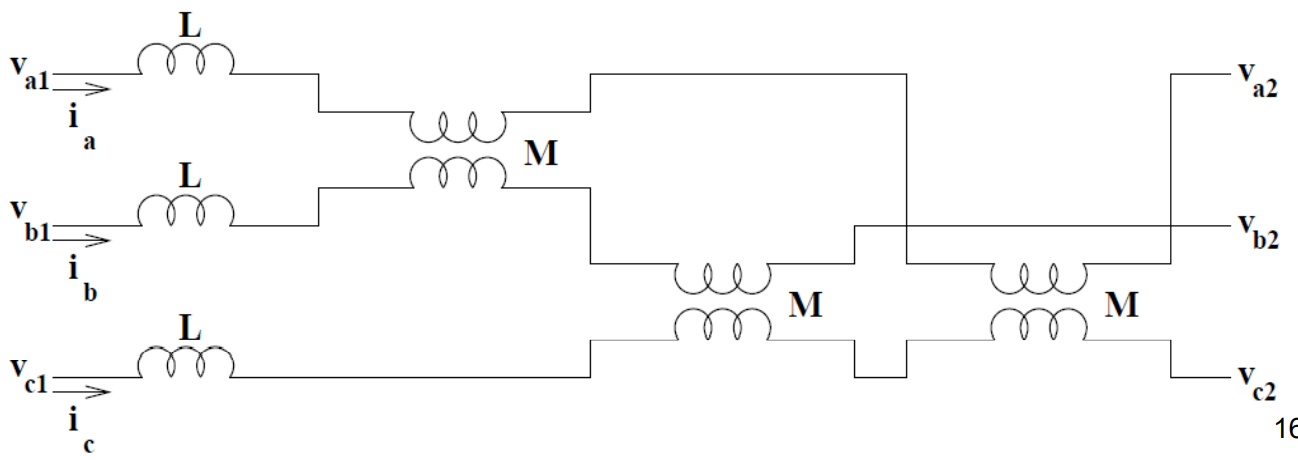
\includegraphics[width = \textwidth]{../img/figure32.png}
	\caption{Trasmission line mutual inductance and self-inductance.}
\end{figure}
\subsection{Transmission line representation}
Hence, we can write the relationship $(V = XI)$: 
\begin{gather}
	\begin{pmatrix}
		V_a\\
		V_b\\
		V_c
	\end{pmatrix} = j \omega \begin{pmatrix}
		L_a & M_{ab} & M_{ac}\\
		M_{ba} & L_b & M_{bc}\\
		M_{ca} & M_{cb} & L_c
	\end{pmatrix}\begin{pmatrix}
		I_a\\
		I_b\\
		I_c
	\end{pmatrix}
\end{gather}
It is reasonable to say that the line and mutual inductances are the same for each transmission line or cable under steady-state balanced conditions. This is not necessarily the case for transient or unbalanced case.
\subsection{Transmission sequence representation}
Bringing in the relationship between phase and sequence components we have (ignoring 1/3):
\begin{gather}
	I_{sequence} = \left[A\right]^{-1} \cdot I_{phase}\\
	V_{sequence} = \left[A\right]^{-1} \cdot V_{phase}
\end{gather}
Hence:
\begin{gather}
	\begin{pmatrix}
		1 & 1 & 1\\
		a^2 & a & 1\\
		a & a^2 & 1
	\end{pmatrix}\begin{pmatrix}
		V_1\\
		V_2\\
		V_3
	\end{pmatrix} = j\omega\begin{pmatrix}
		L_a & M_{ab} & M_{ac}\\
		M_{ba} & L_b & M_{bc}\\
		M_{ca} & M_{cb} & L_c
	\end{pmatrix}\cdot\begin{pmatrix}
		1 & 1 & 1\\
		a^2 & a & 1\\
		a & a^2 & 1
	\end{pmatrix}\begin{pmatrix}
		I_a\\
		I_b\\
		I_c
	\end{pmatrix}\\
	\left[A\right] \left[V_{sequence}\right] = j\omega \left[LM\right]\cdot \left[A\right]\left[I_{sequence}\right]
\end{gather}
\subsection{Transmission line representation}
Hence by transformation we obtain:
\begin{gather}
	\left[V_{sequence}\right] = j\omega\left[A\right]\cdot \left[LM\right]\cdot\left[A\right]^{-1}\left[I_{sequence}\right]
\end{gather}
The part ($\left[A\right]\cdot \left[LM\right]\cdot\left[A\right]^{-1}$) provides the inductance sequence relationship for the transmission line or distribution cable. Resolving gives:
\begin{gather}
	\begin{pmatrix}
		L-M & 0 & 0 \\
		0 & L- M & 0 \\
		0 & 0 & L+2M
	\end{pmatrix}
\end{gather}
The relationship between sequence components becomes:
\begin{gather}
	\begin{pmatrix}
		V_1\\
		V_2\\
		V_3
	\end{pmatrix} = j \omega \begin{pmatrix}
		L-M & 0 & 0 \\
		0 & L- M & 0 \\
		0 & 0 & L+2M
	\end{pmatrix} \begin{pmatrix}
		I_a\\
		I_b\\
		I_c
	\end{pmatrix}
\end{gather}
The sequence component relationships become:
\begin{gather}
	V_1 = j\omega \left(L - M\right)I_1\\
	V_2 = j\omega \left(L - M\right)I_2\\
	V_0 = j\omega \left(L - M\right)I_0
\end{gather}
The positive, negative and zero sequence reactances of the balanced transmission line are then:
\begin{gather}
	Z_1 = Z_2 = j\omega \left(L-M\right) \\
	Z_0 = j\omega \left(L+2M\right)
\end{gather}
\begin{figure}[H]
	\centering
	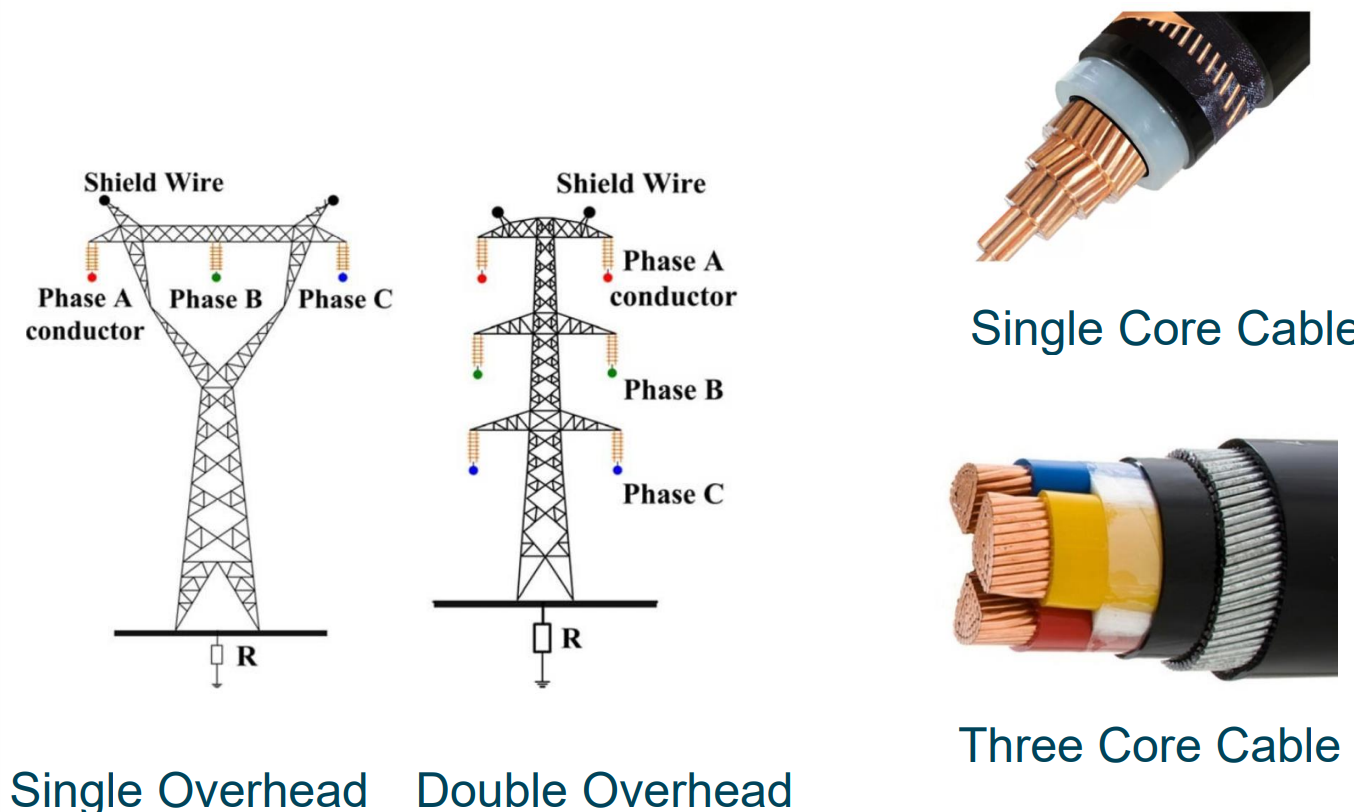
\includegraphics[width = \textwidth]{../img/figure33.png}
	\caption{Transmission line and cable arrangements.}
\end{figure}
\subsection{Lines and cables}
The positive and negative sequence impedances are normally balanced i.e. $Z_1 = Z_2$. The zero sequence impedance depends upon the nature of the return path through the earth. Typical relative values of $Z_0$ during faults are

Overhead:
\begin{itemize}
	\item For a single-circuit arrangement ($Z_0/Z_1$) = 3.5
	\item For a double-circuit arrangement ($Z_0/Z_1$) = 5.5
\end{itemize}
Cable arrangements:
\begin{itemize}
	\item For a single-core arrangement ($Z_0/Z_1$) = 1.25
	\item For a three-core arrangement ($Z_0/Z_1$) = 4
\end{itemize}
\subsection{Synchronous machines (generators)}
The positive sequence reactance $Z_1$ is the value used under balanced operation due to positive sequence currents flowing in the windings of the machine in steady-state and transient. The negative sequence reactance $Z_2$ is due to negative sequence currents which give rise to fluxes in the air gap of the machine that rotate in the opposite direction during unbalance. $Z_2$ is different to $Z_1$ in most designs. The zero sequence reactance $Z_0$ depends upon the nature of the connection of the star point. Zero sequence currents will not flow when the star point is floating but will flow when there is.
\subsection{Neutral connection}
The symmetrical components are independent with the voltage-current relationships:
\begin{gather}
	V_1 = ZI_1\\
	V_2 = ZI_2\\
	V_0 = \left(Z + 3Z_g\right)I_0
\end{gather}
In many generators that are tied to ground at the star point will have additional impedance separately added to reduce the level of zero sequence currents.
\begin{figure}[H]
	\centering
	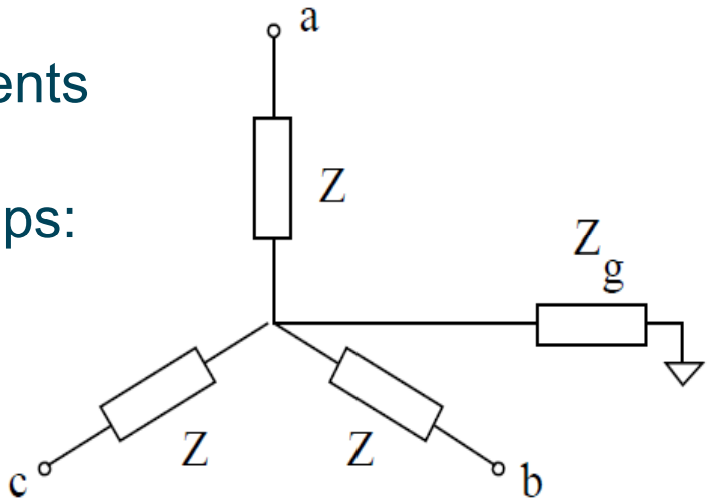
\includegraphics[width = 0.6\textwidth]{../img/figure34.png}
	\caption{Grounded star arrangement.}
\end{figure}
\subsection{Typical values of sequence impedances for synchronous generators}
\begin{table}
	\centering
	\begin{tabular}{@{}llll@{}}
		\toprule
		Type of machine & +ve sequence & -ve sequence & zero sequence\\
		\midrule
		\SI{440}{V} \SI{50}{\hertz} \SI{1}{MVA} & \SI{0.16}{pu} & \SI{0.11}{pu} & \SI{0.05}{pu}\\
		\SI{11}{kV} \SI{50}{\hertz} \SI{75}{MVA} & \SI{0.18}{pu} & \SI{0.14}{pu} & \SI{0.07}{pu}\\ 
		\SI{16}{kV} \SI{50}{\hertz} \SI{275}{MVA} & \SI{0.21}{pu} & \SI{0.18}{pu} & \SI{0.08}{pu}\\ 
		\SI{22}{kV} \SI{50}{\hertz} \SI{575}{MVA} & \SI{0.28}{pu} & \SI{0.21}{pu} & \SI{0.12}{pu}\\
		\bottomrule
	\end{tabular}
	\caption{Table to show typical value of sequence impedances for synchronous generators}
\end{table}
Manufacturers will test their machines to obtain the relevant data/ The value of the sequence components may differ from country to country, manufacturer to manufacturer. 
\subsection{Transformers}
The positive and negative sequence sequence impedances are the normal values obtained from the per-phase equivalent circuit. ($Z_1 = Z_2$). The zero sequence components depend upon the connection of the windings. Zero sequence currents in the windings on one side of the transformer must produce the corresponding ampere-turns in the other. In delta windings the zero-sequence currents circulate through the three-phase windings but do not leave the transformer.
\section{Unbalanced faults}
\subsection{Fortescue's symmetrical component process}
Symmetrical components are used extensively for fault study calculations. in these calculations the positive, negative and zero-sequence impedance networks are either given by the manufacturer or are calculated by the user using base voltages and base power for the system of interest. Each of the sequence networks are then connected together to calculate fault currents and voltages depending upon the type of fault. Standard circuit arrangements have been derived in this course to keep variation reasonable. 
\begin{figure}[H]
	\centering
	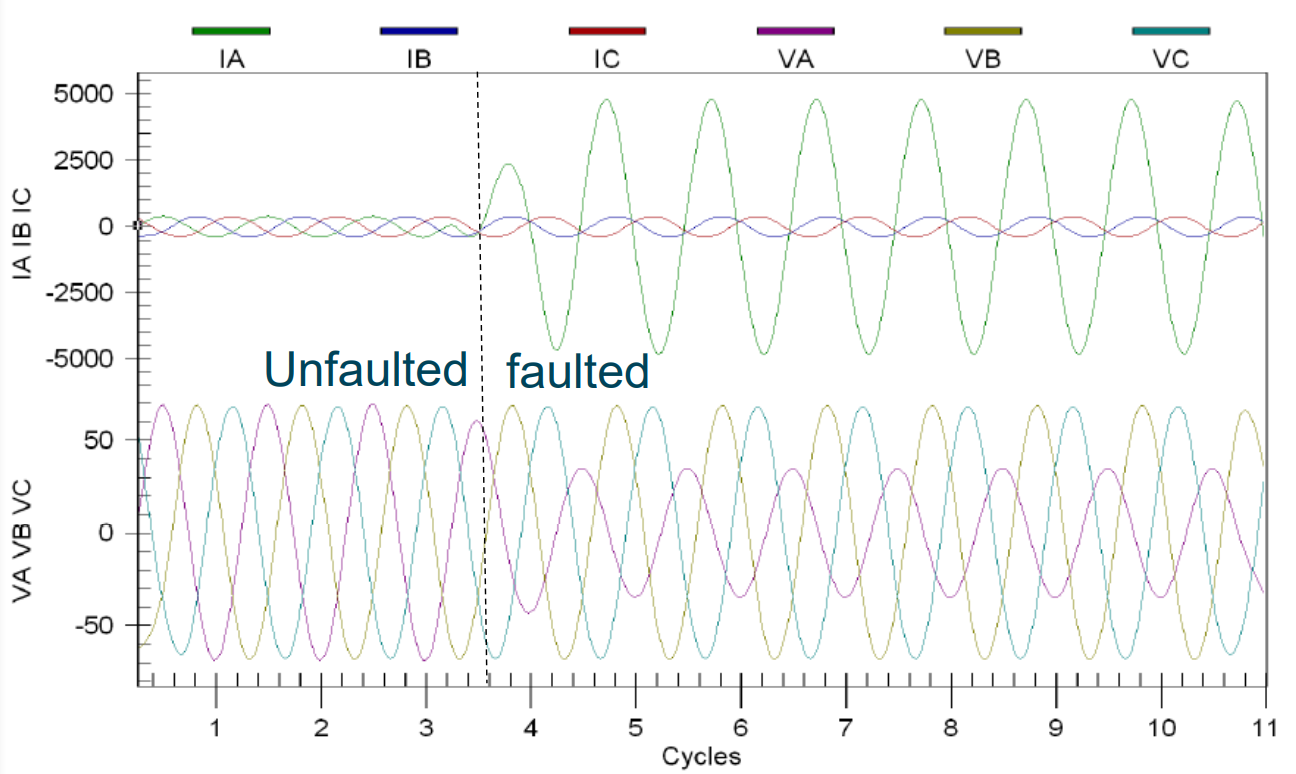
\includegraphics[width = \textwidth]{../img/figure35.png}
	\caption{Line to ground fault.}
\end{figure}
\subsection{Standard fault sequence connections - single line to ground}
\begin{figure}[H]
	\centering
	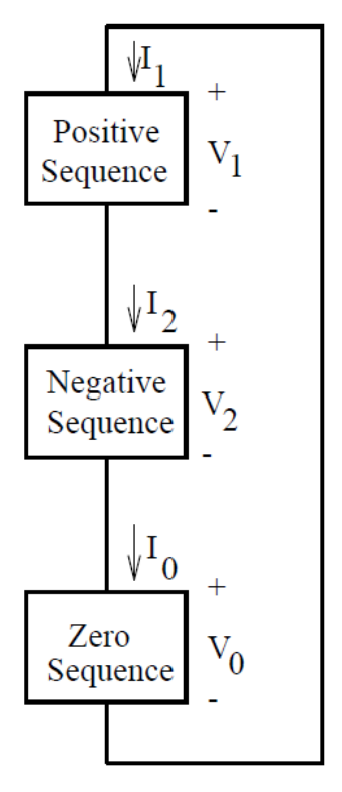
\includegraphics[width = 0.3 \textwidth]{../img/figure36.png}
	\caption{Single line to ground connection.}
\end{figure}
Assumptions:
\begin{itemize}
	\item $V_a = 0$; $I_a$ = very large value (faulted line)
	\item $I_b = 0$ (small in comparision to fault current)
	\item $I_c = 0$ (small in comparision to fault current)
\end{itemize}
Hence for phae voltage `a' we can say:
\begin{gather}
	V_0 + V_1 + V_2 = 0
\end{gather}
And for the current we can say:
\begin{gather}
	I_0 + I_1 + I_2 = \frac{1}{3}I_a
\end{gather}
Together, these two expressions describe the sequence network connection.
\subsection{Standard fault sequence connections - line to line}
\begin{figure}[H]
	\centering
	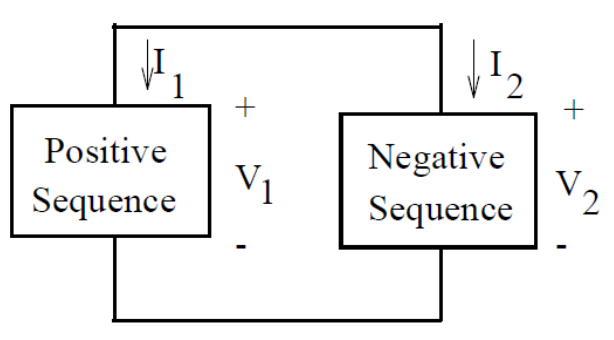
\includegraphics[width = 0.4 \textwidth]{../img/figure37.png}
	\caption{Line to line connection.}
\end{figure}
Assumptions. If the fault occurs between phase b and c then we can say:
\begin{itemize}
	\item $V_b = V_c$
	\item $I_b = -I_c$
	\item $I_a = 0$ (since it is small in comparison with the fault current)
\end{itemize}
Hence, we can use the phase sequence relationships to say:
\begin{gather}
	V_1 = V_2 \textrm{ and also } I_a = I_1 + I_2 \textrm{ since } I_0 = 0
\end{gather}
\subsection{Standard fault sequence connections - double line to ground}
\begin{figure}[H]
	\centering
	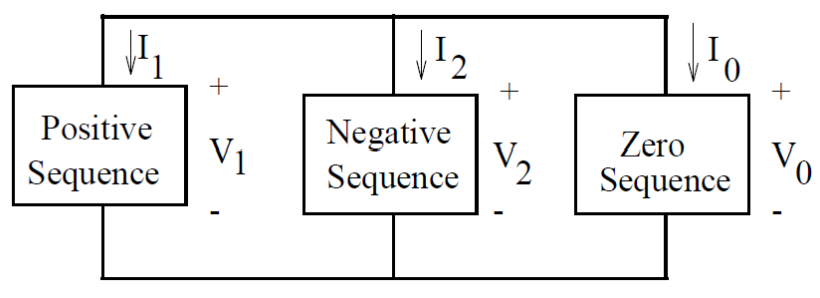
\includegraphics[width = 0.7\textwidth]{../img/figure38.png}
	\caption{Double line to ground connection.}
\end{figure}
Assumptions. If the fault involves phases b and c to ground then we can say:
\begin{itemize}
	\item $I_a = 0$ (small in comparison to fault current)
	\item $V_b = 0$ (faulted line)
	\item $V_c = 0$ (faulted line)
\end{itemize}
Hence using phase-sequence relationships we can further say that:
\begin{gather}
	V_0 + V_1 + V_2 = 0\\
	I_a = I_0 + I_1 + I_2 = 0
\end{gather}
\section{A full fault analysis study}
\subsection{Breaker sizing method (most common approach)}
One of the main purposes of circuit breakers is to arrest large currents that flow when there is a fault. Breaker sizing is achieved by understanding currents flowing under both symmetrical and non-symmetrical fault conditions (to be calculated). Calculations are carried out using symmetrical components i.e. positive, negative and zero sequence. Only one phae needs to be considered \dots but all fault types need to be calculated.
\subsection{Breaker sizing example}
Determine the maximum current through the breaker B due to a fault at the location X. Calculate all three types of unbalanced fult and the balanced fault currents. 
\begin{itemize}
	\item System base: voltage \SI{138}{kV} (\SI{1}{pu}), Power \SI{100}{MVA} (\SI{1}{pu})
	\item Transformer $T_1$ leakage reactance j0.1 pu
	\item Transformer $T_2$ leakage reactance j0.1 pu
	\item Line L1: positive and negative sequence reactance j0.05 pu, zero sequence reactance j0.1 pu
	\item Line L2: positive and negative sequence reactance j0.02 pu, zero sequence reactance j0.1 pu
\end{itemize}
\begin{figure}[H]
	\centering
	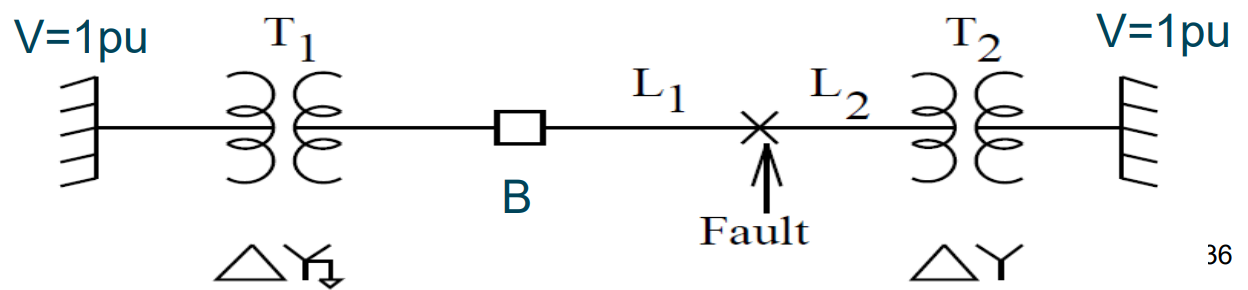
\includegraphics[width = \textwidth]{../img/figure39.png}
	\caption{Breaker sizing example.}
\end{figure}
\subsection{Sequence component arrangement}
\begin{figure}[H]
	\centering
	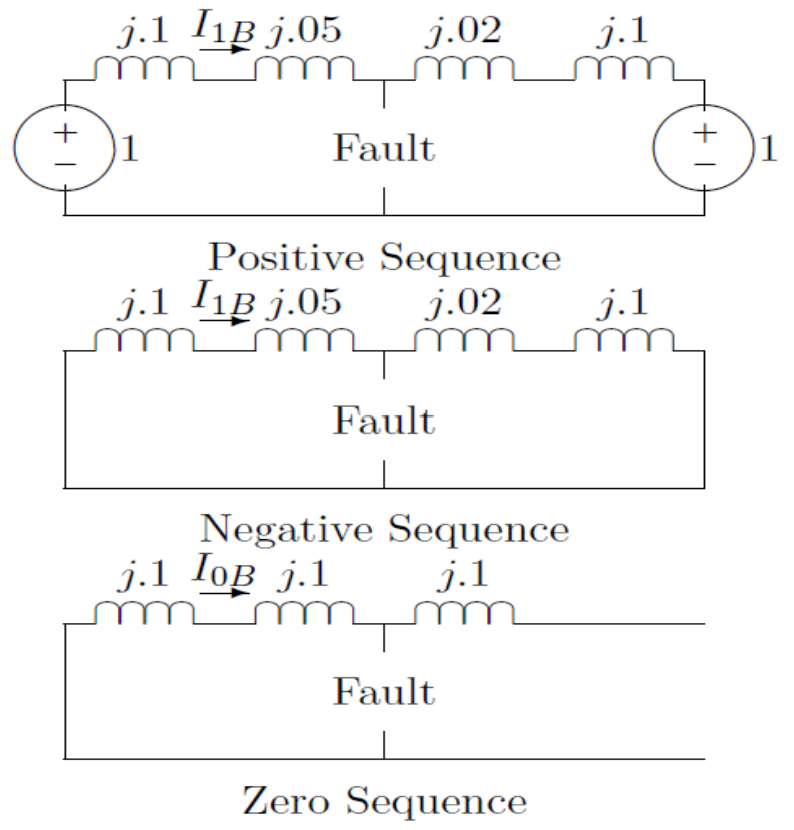
\includegraphics[width = 0.5\textwidth]{../img/figure40.png}
	\caption{Sequence component arrangement.}
\end{figure}
The sequence networks are exactly like what we would expect to have drawn for equivalent single phase networks. A positive, negative and zero sequence arrangmenet has been shown for one phase. Only the positive sequence network has sources, because the infinite bus supplies only positive sequence voltage. The zero sequence network is open at the right hand side because of the delta-wye transformer connection.
\subsection{Symmetrical fault current}
For a symmetrical (three-phase) fault, only the positive sequence network is involved. The fault shorts the network at its position, so that the current is:
\begin{gather}
	I_1 = \frac{1}{j0.15} - j6.67 \textrm{ per unit from LHS}\\
	(I_1 = \frac{1}{j0.12} - j8.33 \textrm{ per unit from RHS})
\end{gather}
\begin{figure}[H]
	\centering
	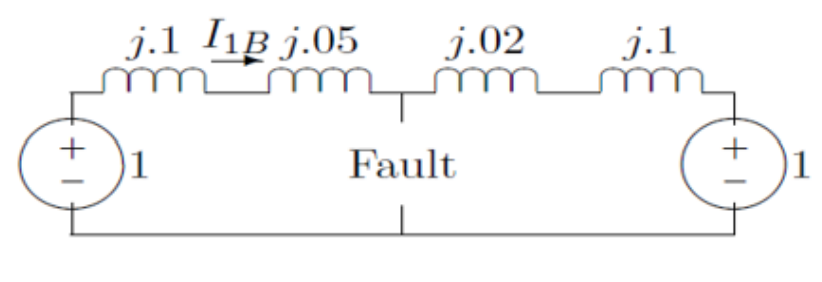
\includegraphics[width = 0.8\textwidth]{../img/figure41.png}
	\caption{Positive sequence impedance in symmetrical fault.}
\end{figure}
\subsection{Single line to ground fault}
\begin{figure}[H]
	\centering
	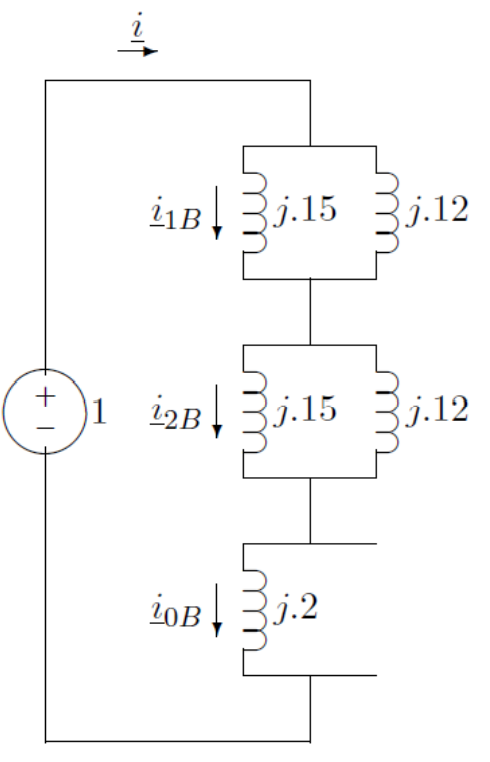
\includegraphics[width = 0.4\textwidth]{../img/figure42.png}
	\caption{Positive sequence impedance in symmetrical fault.}
\end{figure}
The three networks are in series and the situation is as shown with the total current given by:
\begin{gather}
	\underline{i} = \frac{1}{2 \times \left(j0.15 || j0.12\right) + j0.2} = -j3.0
\end{gather}
The sequence currents are:
\begin{align}
	\underline{i}_{1B} &= \underline{i}_{2B}\\
	&= \underline{i} \times \frac{j0.12}{j0.12 + j0.15}\\
	&= -j1.33
	\underline{i}_{0B} &= \underline{i}\\
	&= -j3.0
\end{align}
\subsection{Singe line to ground fault}
Having calculated the sequence currents, the phase currents can be reconstructed:
\begin{align}
	\underline{i}_a &= \underline{i}_{1B} + \underline{i}_{2B} + \underline{i}_{0B}\\
	\underline{i}_b &= \underline{a^2i}_{1B} + \underline{ai}_{2B} + \underline{i}_{0B}\\
	\underline{i}_c &= \underline{ai}_{1B} + \underline{a^2i}_{2B} + \underline{i}_{0B}
\end{align}
Hence:
\begin{align}
	\underline{i}_a &= -j5.66\, \textrm{pu}\\
	\underline{i}_b &= -j1.67\, \textrm{pu}\\
	\underline{i}_c &= -j1.67\, \textrm{pu}
\end{align}
\subsection{Double line to ground fault}
\begin{figure}[H]
	\centering
	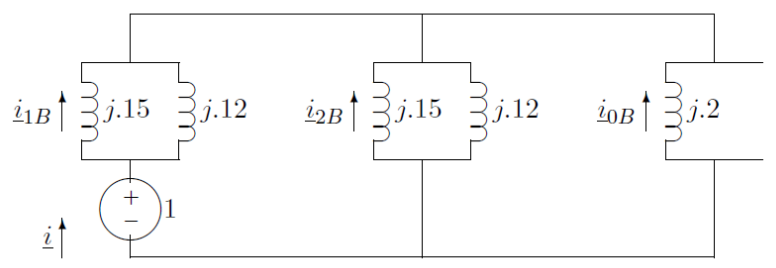
\includegraphics[width = \textwidth]{../img/figure43.png}
	\caption{Double line-ground fault configuration.}
\end{figure}
For the double line-ground fault, the networks are in parallel.
\begin{align}
	\underline{i} &= \frac{1}{j\left(0.15||0.12\right)+ j \left(0.15||0.12||0.2\right)}\\
	&= -j8.57\\
	\underline{i}_{1B} &= \underline{i} \times \frac{j0.12}{j0.12 + j0.15}\\
	&= -j3.81\\
	\underline{i}_{2B} &= -\underline{i} \times \frac{j0.12 ||j0.2}{j0.12||j0.2 + j0.15}\\
	&= j2.86\\
	\underline{i}_{0B} &= \underline{i}\times \frac{j0.12||j0.15}{j0.2 + j0.12||j0.15}\\
	&= j2.14
\end{align}
Having calculated the sequence currents, the phase currents can be reconstructed:
\begin{align}
	\underline{i}_a &= j1.19\\
	\underline{i}_b &= \underline{i}_{0B} - \frac{1}{2}\left(\underline{i}_{1B} + \underline{i}_{2B}\right)-\frac{\sqrt{3}}{2}j\left(\underline{i}_{1B} - \underline{i}_{2B}\right)\\
	&= j2.67 - 5.87\\
	\underline{i}_c &= \underline{i}_{0B} - \frac{1}{2}\left(\underline{i}_{1B}+\underline{i}_{2B}\right) + \frac{\sqrt{3}}{2} j \left(\underline{i}_{1B} - \underline{i}_{2B}\right)\\
	&= j2.67 + 5.87
\end{align}
Hence:
\begin{align}
	\left| \underline{i}_{a}\right| &= 1.19\, \textrm{pu}\\
	\left| \underline{i}_{b}\right| &= 6.43\, \textrm{pu}\\
	\left| \underline{i}_{c}\right| &= 6.43\, \textrm{pu}
\end{align}
\subsection{Line to line fault}
Having calculated the sequence currents, the phase currents can be reconstructed:
\begin{align}
	\underline{i}_a &= 0\\
	\underline{i}_b &= -\frac{1}{2}\left(\underline{i}_{1B}+ \underline{i}_{2B}\right) - j\frac{\sqrt{3}}{2}\left(\underline{i}_{1B}-\underline{i}_{2B}\right)
\end{align}
Hence:
\begin{align}
	\left|\underline{i}_{b}\right| &= 5.77\, \textrm{pu}\\
	\left|\underline{i}_{c}\right| &= 5.77\, \textrm{pu}
\end{align}
There are only two networks at play - positive and negative sequence.
\begin{figure}[H]
	\centering
	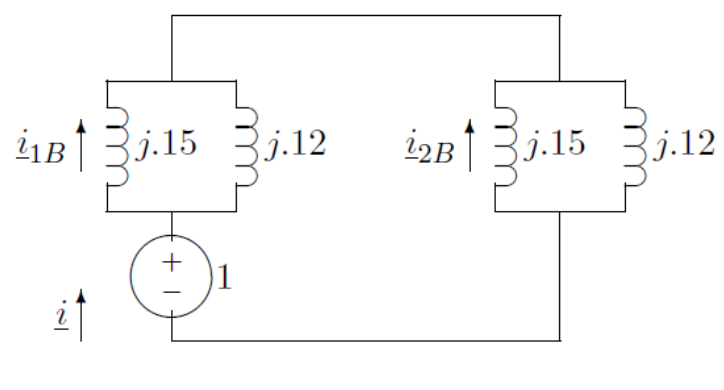
\includegraphics[width = 0.5\textwidth]{../img/figure44.png}
	\caption{Line to line fault configuration.}
\end{figure}
\subsection{Conversion to ampere ratings}
Having calculated the fault currents then the values in per unit can be expressed as amperes. The value of $I_B$ is:
\begin{gather}
	I_B = \frac{P_B}{\sqrt{3}V_{Bl-l}} = \SI{418.8}{A}
\end{gather}
Hence the fault currents are calculated as being:
\begin{table}
	\centering
	\begin{tabular}{@{}llll@{}}
		\toprule
		& Phase A & Phase B & Phase C\\
		\midrule
		Three-phase fault & 2791 & 2791 & 2791\\
		Single line-ground, $\phi_a$ & 2368 & 699 & 699\\
		Double line-ground, $\phi_b$, $\phi_c$ & 498 & 2690 & 2690\\
		Line-line, $\phi_b$, $\phi_c$ & 0 & 2414 & 2414\\
		\bottomrule
	\end{tabular}
	\caption{Table to show fault currents.}
\end{table}
The worst fault is the balanced three-phase fault.
\subsection{Practical sizing of breakers}
Key information needed for sizing a circuit breaker include:
\begin{itemize}
	\item Voltage rating
	\item Normal current rating
	\item MVA fault level
	\item Fault current levels
	\item Withstand voltage levels
\end{itemize}
There are three main types of circuit breakers: Air, vacuum and SF6. 
\subsection{Conclusions}
\begin{itemize}
	\item Appreciated the need for positive, negative and zero sequence impedances of different components to make up a power system
	\item Introduced the concept of positive, negative and zero sequence impedance. Examined this at a component level
	\item A system analysis method has been applied for `unbalanced faults' in a transmission system and fault current table produced
\end{itemize}
\end{document}